\documentclass[ignorenonframetext, 10pt, aspectratio=169]{beamer}

\usepackage{kuriwaki_pream}


\title{\textbf{\large{\texttt{svysim}:\\Creating Realistic Simulations of (Biased) Survey Data}}}
\author{Shiro Kuriwaki}
\date{\small\today}


\begin{document}

% TITLE ----------
\begin{frame}
\centering
\maketitle
\url{https://github.com/kuriwaki/svysim}
\end{frame}

\begin{frame}
{Motivation: Existing simulations of survey response are too simplistic}


\begin{columns}
\begin{column}{0.7\linewidth}
Simulated data are important for demonstrating predictive accuracy and proper coverage of estimators, but existing simulations ...
\medskip
\begin{wideitemize}
\item Use continuous predictors, but almost all survey data is categorical
\item Assume no multilevel / clustering structure
\item Assume no selection bias
\end{wideitemize}

\bigskip
\rightfoot{(for exceptions, see \href{https://mc-stan.org/rstanarm/articles/mrp.html}{Kennedy and Gabry})}

\end{column}
\end{columns}

\end{frame}


\begin{frame}
{Package \texttt{svysim}: Realistic simulation, with control over the sampling scheme}

\begin{columns}
\begin{column}{0.7\linewidth}
\begin{wideitemize}
	\item Population ($N = 600,000$): CCES Data, expanded using post-stratification weights
	\begin{itemize}
	\item This is technically not a census, but it has a natural covariance structure and makes the simulation realistic.
	\end{itemize}
	\item Sample ($n = 1,000$): Simple Random Sample (SRS), OR a biased sample where the propensity score for population member \(i \in \{1, ..., N\}\) is determined by a propensity score \(p_i\).
	\item Then I get a sample by: \texttt{sample(1:N, size = n, replace = FALSE, prob =} Propensity Score$_i$\texttt{)}
\end{wideitemize}
\end{column}
\end{columns}


\end{frame}

\begin{frame}
{Sampling Functions}

\(p_i = \text{invlogit}(bX)\) where 

\bigskip

``High Education'': here \(bX\) is:

\small
\begin{align*}
 = \left\{-4 + 2\text{Urban}_i + \begin{bmatrix}1.0\\0.8 \\0.7\\ 0.6\\ 0.5\end{bmatrix}^\top\begin{bmatrix}\text{White}_i\\\text{Black}_i\\\text{Hispanic}_i\\\text{Asian}_i\\\text{All Other}_i\\\end{bmatrix} + 
\begin{bmatrix}4.0\\3.0\\1.2\\0.5\end{bmatrix}^\top\begin{bmatrix}\text{Post-Grad}_i\\\text{4-Year}_i\\\text{Some College}_i\\\text{HS or Less}_i\end{bmatrix}  + 
\begin{bmatrix}4.0\\1.0\\ 0.4\\ 0.3\end{bmatrix}^\top\begin{bmatrix}\text{Follow News}_i\\\text{Sometimes}_i\\\text{Now and Then}_i\\\text{Hardly}_i\end{bmatrix}\right\}
\end{align*}
\normalsize
where e.g. White$_{i}$ is an indicator variable for whether respondent \(i\) is White. 

\bigskip


``High Ed + Partisanship'' adds the following partisan component to \(bX\):
\small
\begin{align*}
-2 + \begin{bmatrix}1.25\\0.75\\1\end{bmatrix}^\top\begin{bmatrix}\text{Dem}_{i}\\\text{Indep}_i\\\text{GOP}_i\end{bmatrix}
\end{align*}
\end{frame}


\begin{frame}
{Simulated Outcome}
\begin{align*}
Y_i =& \frac{1}{10}(-3 + A_i + 0.2 B_i + 0.8 C_i + u_i)\\
Z_i =& \text{ invlogit}(Y_i)
\end{align*}

where:
\begin{align*}
A_i &= 0.5\log(\text{Age}_i) -2\mathds{1}(\text{White Male Non-Postgrad}_i) + 2(\text{Follow News}_i) + \begin{bmatrix}0\\1.5\\-0.5\end{bmatrix}^\top\begin{bmatrix}\text{Dem}_{i}\\\text{Indep}_i\\\text{GOP}_i\end{bmatrix}\\
B_i &\sim \text{Bern}(\pi_{\text{state}[i]}), \text{ such that }  ICC = 0.15\\
C_i &\sim \text{Bern}(\pi_{\text{district}[i]}), \text{ such that }  ICC = 0.3\\
u_i &\sim \mathcal{t}(0, \text{df} = 5)
\end{align*}

\normalsize
in which \(\pi_{\text{state}[i]}\) is the state-level average of \(\text{invlogit}(Y_i)\), and ICC is the intraclass cluster coefficient


\end{frame}

\begin{frame}
{Strong error when sampling explicitly is a function of outcome}

\centering
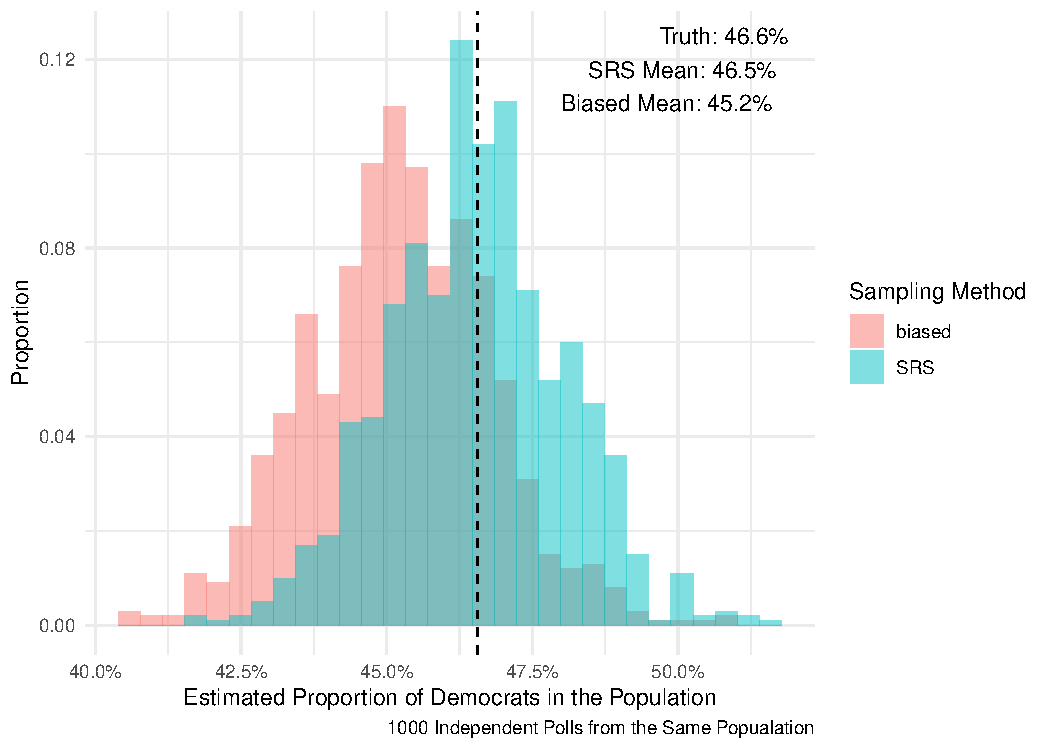
\includegraphics[width =0.8\linewidth]{sampling.png}
\end{frame}

\end{document}
